\documentclass{beamer}
\usepackage[utf8]{inputenc}
\usepackage{hyperref}
\usepackage{enumerate}
\usepackage{graphicx}
\graphicspath{{./images/}}
\usetheme{Warsaw}
\usecolortheme{whale}
\newcommand{\Aiden}{Aiden Taylor - B.Sc. in Computer Science}
\newcommand{\Noah}{Noah Pinel - B.Sc. in Computer Science}
\newcommand{\Ty}{Ty Irving - B.Sc. in Computer Science}
\setbeamertemplate{page number in head/foot}[framenumber]
%\setbeamertemplate{headline}{}

\begin{document}
\title[CPSC 530]{The Implementation and Comparison of the BCCBT Data Compression Algorithm}
\author[Group 17]{
\begin{tabular}{l}
    \Aiden \\ \Noah\\ \Ty\\ 
\end{tabular}}
\date{Apr. 11th, 2023}

\begingroup
    \setbeamertemplate{headline}{}
    \frame{\titlepage}
\endgroup

\begin{frame}
    \tableofcontents
\end{frame}

\section{Quiz Questions}
\begin{frame}
\begin{enumerate}[1.]
\item What specific type of Binary Tree is used in the implementation of the BCCBT Data Compression Algorithm?
Describe at least one discussed property of this type of Binary Tree.
\item Given the specific binary tree needed for the BCCBT algorithm, where the 
tree's nodes correspond to symbols in an arbitrary alphabet $\Sigma$.
Denote a symbol $\phi$, such that $\phi$ is in our arbitrary alphabet $\Sigma$.
Note, $\phi$ is \textbf{NOT} the root of the tree.\\
How is the bit code generated for the symbol $\phi$?
\item Does the BCCBT Data Compression Algorithm make use of the frequency/probability
of each unique symbol in the source file? Explain why or why not.
\end{enumerate}
\end{frame}


\section{Pseudocode}
\begin{frame}
\begin{center}
Bit Code Complete Binary Tree (BCCBT)
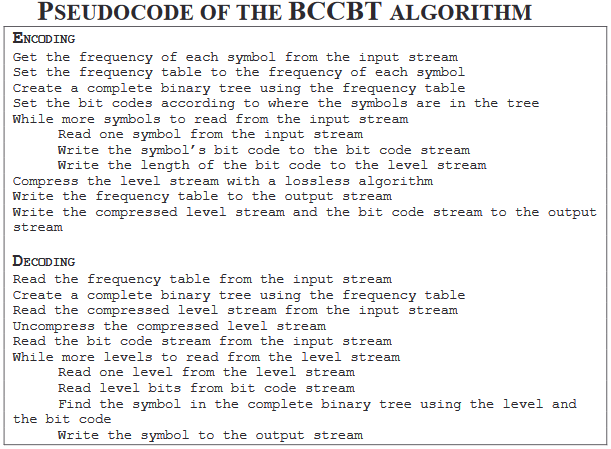
\includegraphics[scale=0.55]{pseudocode}
\end{center}
\end{frame}

\section{Example}
\begin{frame}
\begin{center}
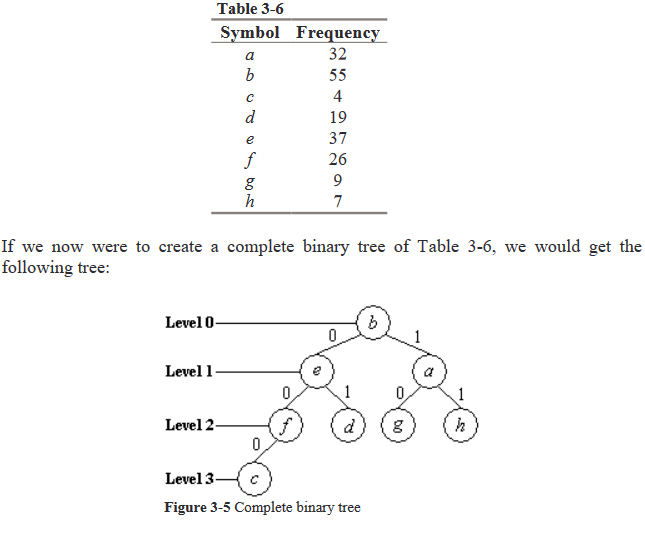
\includegraphics[scale=0.55]{example}
\end{center}
\end{frame}

\subsection{Complete Binary Trees and Frequencies}
\begin{frame}
Properties of Complete Binary Trees:
\begin{itemize}
\item All levels are completely full except possibly the lowest level.
\item Filled from left to right at each level. i.e. Tree leans left.
\item The number of nodes at level $n$ is $2^n$.
\end{itemize}
\end{frame}

\begin{frame}
\begin{center}
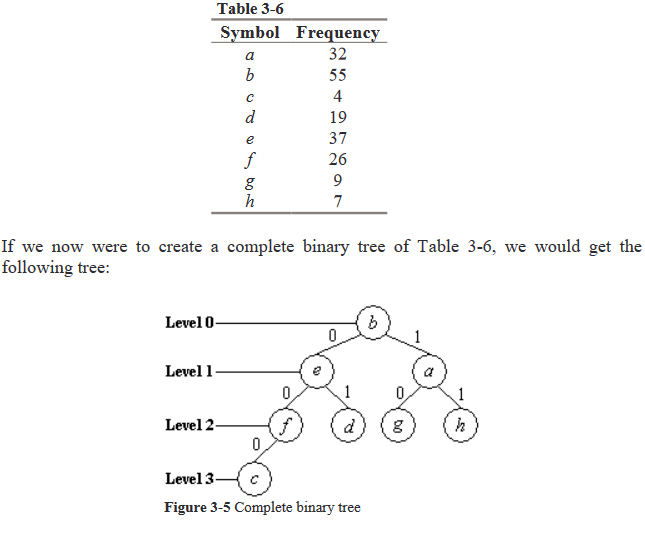
\includegraphics[scale=0.55]{example}
\end{center}
\end{frame}

\subsection{Encoding and Decoding}
\begin{frame}
Hello
\end{frame}

\section{Test Results}
\begin{frame}
Hello
\end{frame}

\section{Q\&A}
\begin{frame}
Hello
\end{frame}

\end{document}
